\documentclass[a4paper,11pt,final]{article}
        \usepackage{fancyvrb, color, graphicx, hyperref, amsmath, url, textcomp}
        \usepackage{palatino}
        \usepackage[a4paper,text={16.5cm,25.2cm},centering]{geometry}

        %Set different options for xetex and luatex
        \usepackage{iftex}
        \ifxetex\usepackage{fontspec}\fi

        \ifluatex\usepackage{fontspec}\fi

        \usepackage{xcolor}
        % ANSI colors from nbconvert
        \definecolor{ansi-black}{HTML}{3E424D}
        \definecolor{ansi-black-intense}{HTML}{282C36}
        \definecolor{ansi-red}{HTML}{E75C58}
        \definecolor{ansi-red-intense}{HTML}{B22B31}
        \definecolor{ansi-green}{HTML}{00A250}
        \definecolor{ansi-green-intense}{HTML}{007427}
        \definecolor{ansi-yellow}{HTML}{DDB62B}
        \definecolor{ansi-yellow-intense}{HTML}{B27D12}
        \definecolor{ansi-blue}{HTML}{208FFB}
        \definecolor{ansi-blue-intense}{HTML}{0065CA}
        \definecolor{ansi-magenta}{HTML}{D160C4}
        \definecolor{ansi-magenta-intense}{HTML}{A03196}
        \definecolor{ansi-cyan}{HTML}{60C6C8}
        \definecolor{ansi-cyan-intense}{HTML}{258F8F}
        \definecolor{ansi-white}{HTML}{C5C1B4}
         \definecolor{ansi-white-intense}{HTML}{A1A6B2}

        \hypersetup
        {   pdfauthor = {Pweave},
            pdftitle={Published from p3.py},
            colorlinks=TRUE,
            linkcolor=black,
            citecolor=blue,
            urlcolor=blue
        }
        \setlength{\parindent}{0pt}
        \setlength{\parskip}{1.2ex}
        % fix for pandoc 1.14
        \providecommand{\tightlist}{%
            \setlength{\itemsep}{0pt}\setlength{\parskip}{0pt}}
        
\makeatletter
\def\PY@reset{\let\PY@it=\relax \let\PY@bf=\relax%
    \let\PY@ul=\relax \let\PY@tc=\relax%
    \let\PY@bc=\relax \let\PY@ff=\relax}
\def\PY@tok#1{\csname PY@tok@#1\endcsname}
\def\PY@toks#1+{\ifx\relax#1\empty\else%
    \PY@tok{#1}\expandafter\PY@toks\fi}
\def\PY@do#1{\PY@bc{\PY@tc{\PY@ul{%
    \PY@it{\PY@bf{\PY@ff{#1}}}}}}}
\def\PY#1#2{\PY@reset\PY@toks#1+\relax+\PY@do{#2}}

\expandafter\def\csname PY@tok@w\endcsname{\def\PY@tc##1{\textcolor[rgb]{0.73,0.73,0.73}{##1}}}
\expandafter\def\csname PY@tok@c\endcsname{\let\PY@it=\textit\def\PY@tc##1{\textcolor[rgb]{0.25,0.50,0.50}{##1}}}
\expandafter\def\csname PY@tok@cp\endcsname{\def\PY@tc##1{\textcolor[rgb]{0.74,0.48,0.00}{##1}}}
\expandafter\def\csname PY@tok@k\endcsname{\let\PY@bf=\textbf\def\PY@tc##1{\textcolor[rgb]{0.00,0.50,0.00}{##1}}}
\expandafter\def\csname PY@tok@kp\endcsname{\def\PY@tc##1{\textcolor[rgb]{0.00,0.50,0.00}{##1}}}
\expandafter\def\csname PY@tok@kt\endcsname{\def\PY@tc##1{\textcolor[rgb]{0.69,0.00,0.25}{##1}}}
\expandafter\def\csname PY@tok@o\endcsname{\def\PY@tc##1{\textcolor[rgb]{0.40,0.40,0.40}{##1}}}
\expandafter\def\csname PY@tok@ow\endcsname{\let\PY@bf=\textbf\def\PY@tc##1{\textcolor[rgb]{0.67,0.13,1.00}{##1}}}
\expandafter\def\csname PY@tok@nb\endcsname{\def\PY@tc##1{\textcolor[rgb]{0.00,0.50,0.00}{##1}}}
\expandafter\def\csname PY@tok@nf\endcsname{\def\PY@tc##1{\textcolor[rgb]{0.00,0.00,1.00}{##1}}}
\expandafter\def\csname PY@tok@nc\endcsname{\let\PY@bf=\textbf\def\PY@tc##1{\textcolor[rgb]{0.00,0.00,1.00}{##1}}}
\expandafter\def\csname PY@tok@nn\endcsname{\let\PY@bf=\textbf\def\PY@tc##1{\textcolor[rgb]{0.00,0.00,1.00}{##1}}}
\expandafter\def\csname PY@tok@ne\endcsname{\let\PY@bf=\textbf\def\PY@tc##1{\textcolor[rgb]{0.82,0.25,0.23}{##1}}}
\expandafter\def\csname PY@tok@nv\endcsname{\def\PY@tc##1{\textcolor[rgb]{0.10,0.09,0.49}{##1}}}
\expandafter\def\csname PY@tok@no\endcsname{\def\PY@tc##1{\textcolor[rgb]{0.53,0.00,0.00}{##1}}}
\expandafter\def\csname PY@tok@nl\endcsname{\def\PY@tc##1{\textcolor[rgb]{0.63,0.63,0.00}{##1}}}
\expandafter\def\csname PY@tok@ni\endcsname{\let\PY@bf=\textbf\def\PY@tc##1{\textcolor[rgb]{0.60,0.60,0.60}{##1}}}
\expandafter\def\csname PY@tok@na\endcsname{\def\PY@tc##1{\textcolor[rgb]{0.49,0.56,0.16}{##1}}}
\expandafter\def\csname PY@tok@nt\endcsname{\let\PY@bf=\textbf\def\PY@tc##1{\textcolor[rgb]{0.00,0.50,0.00}{##1}}}
\expandafter\def\csname PY@tok@nd\endcsname{\def\PY@tc##1{\textcolor[rgb]{0.67,0.13,1.00}{##1}}}
\expandafter\def\csname PY@tok@s\endcsname{\def\PY@tc##1{\textcolor[rgb]{0.73,0.13,0.13}{##1}}}
\expandafter\def\csname PY@tok@sd\endcsname{\let\PY@it=\textit\def\PY@tc##1{\textcolor[rgb]{0.73,0.13,0.13}{##1}}}
\expandafter\def\csname PY@tok@si\endcsname{\let\PY@bf=\textbf\def\PY@tc##1{\textcolor[rgb]{0.73,0.40,0.53}{##1}}}
\expandafter\def\csname PY@tok@se\endcsname{\let\PY@bf=\textbf\def\PY@tc##1{\textcolor[rgb]{0.73,0.40,0.13}{##1}}}
\expandafter\def\csname PY@tok@sr\endcsname{\def\PY@tc##1{\textcolor[rgb]{0.73,0.40,0.53}{##1}}}
\expandafter\def\csname PY@tok@ss\endcsname{\def\PY@tc##1{\textcolor[rgb]{0.10,0.09,0.49}{##1}}}
\expandafter\def\csname PY@tok@sx\endcsname{\def\PY@tc##1{\textcolor[rgb]{0.00,0.50,0.00}{##1}}}
\expandafter\def\csname PY@tok@m\endcsname{\def\PY@tc##1{\textcolor[rgb]{0.40,0.40,0.40}{##1}}}
\expandafter\def\csname PY@tok@gh\endcsname{\let\PY@bf=\textbf\def\PY@tc##1{\textcolor[rgb]{0.00,0.00,0.50}{##1}}}
\expandafter\def\csname PY@tok@gu\endcsname{\let\PY@bf=\textbf\def\PY@tc##1{\textcolor[rgb]{0.50,0.00,0.50}{##1}}}
\expandafter\def\csname PY@tok@gd\endcsname{\def\PY@tc##1{\textcolor[rgb]{0.63,0.00,0.00}{##1}}}
\expandafter\def\csname PY@tok@gi\endcsname{\def\PY@tc##1{\textcolor[rgb]{0.00,0.63,0.00}{##1}}}
\expandafter\def\csname PY@tok@gr\endcsname{\def\PY@tc##1{\textcolor[rgb]{1.00,0.00,0.00}{##1}}}
\expandafter\def\csname PY@tok@ge\endcsname{\let\PY@it=\textit}
\expandafter\def\csname PY@tok@gs\endcsname{\let\PY@bf=\textbf}
\expandafter\def\csname PY@tok@gp\endcsname{\let\PY@bf=\textbf\def\PY@tc##1{\textcolor[rgb]{0.00,0.00,0.50}{##1}}}
\expandafter\def\csname PY@tok@go\endcsname{\def\PY@tc##1{\textcolor[rgb]{0.53,0.53,0.53}{##1}}}
\expandafter\def\csname PY@tok@gt\endcsname{\def\PY@tc##1{\textcolor[rgb]{0.00,0.27,0.87}{##1}}}
\expandafter\def\csname PY@tok@err\endcsname{\def\PY@bc##1{\setlength{\fboxsep}{0pt}\fcolorbox[rgb]{1.00,0.00,0.00}{1,1,1}{\strut ##1}}}
\expandafter\def\csname PY@tok@kc\endcsname{\let\PY@bf=\textbf\def\PY@tc##1{\textcolor[rgb]{0.00,0.50,0.00}{##1}}}
\expandafter\def\csname PY@tok@kd\endcsname{\let\PY@bf=\textbf\def\PY@tc##1{\textcolor[rgb]{0.00,0.50,0.00}{##1}}}
\expandafter\def\csname PY@tok@kn\endcsname{\let\PY@bf=\textbf\def\PY@tc##1{\textcolor[rgb]{0.00,0.50,0.00}{##1}}}
\expandafter\def\csname PY@tok@kr\endcsname{\let\PY@bf=\textbf\def\PY@tc##1{\textcolor[rgb]{0.00,0.50,0.00}{##1}}}
\expandafter\def\csname PY@tok@bp\endcsname{\def\PY@tc##1{\textcolor[rgb]{0.00,0.50,0.00}{##1}}}
\expandafter\def\csname PY@tok@fm\endcsname{\def\PY@tc##1{\textcolor[rgb]{0.00,0.00,1.00}{##1}}}
\expandafter\def\csname PY@tok@vc\endcsname{\def\PY@tc##1{\textcolor[rgb]{0.10,0.09,0.49}{##1}}}
\expandafter\def\csname PY@tok@vg\endcsname{\def\PY@tc##1{\textcolor[rgb]{0.10,0.09,0.49}{##1}}}
\expandafter\def\csname PY@tok@vi\endcsname{\def\PY@tc##1{\textcolor[rgb]{0.10,0.09,0.49}{##1}}}
\expandafter\def\csname PY@tok@vm\endcsname{\def\PY@tc##1{\textcolor[rgb]{0.10,0.09,0.49}{##1}}}
\expandafter\def\csname PY@tok@sa\endcsname{\def\PY@tc##1{\textcolor[rgb]{0.73,0.13,0.13}{##1}}}
\expandafter\def\csname PY@tok@sb\endcsname{\def\PY@tc##1{\textcolor[rgb]{0.73,0.13,0.13}{##1}}}
\expandafter\def\csname PY@tok@sc\endcsname{\def\PY@tc##1{\textcolor[rgb]{0.73,0.13,0.13}{##1}}}
\expandafter\def\csname PY@tok@dl\endcsname{\def\PY@tc##1{\textcolor[rgb]{0.73,0.13,0.13}{##1}}}
\expandafter\def\csname PY@tok@s2\endcsname{\def\PY@tc##1{\textcolor[rgb]{0.73,0.13,0.13}{##1}}}
\expandafter\def\csname PY@tok@sh\endcsname{\def\PY@tc##1{\textcolor[rgb]{0.73,0.13,0.13}{##1}}}
\expandafter\def\csname PY@tok@s1\endcsname{\def\PY@tc##1{\textcolor[rgb]{0.73,0.13,0.13}{##1}}}
\expandafter\def\csname PY@tok@mb\endcsname{\def\PY@tc##1{\textcolor[rgb]{0.40,0.40,0.40}{##1}}}
\expandafter\def\csname PY@tok@mf\endcsname{\def\PY@tc##1{\textcolor[rgb]{0.40,0.40,0.40}{##1}}}
\expandafter\def\csname PY@tok@mh\endcsname{\def\PY@tc##1{\textcolor[rgb]{0.40,0.40,0.40}{##1}}}
\expandafter\def\csname PY@tok@mi\endcsname{\def\PY@tc##1{\textcolor[rgb]{0.40,0.40,0.40}{##1}}}
\expandafter\def\csname PY@tok@il\endcsname{\def\PY@tc##1{\textcolor[rgb]{0.40,0.40,0.40}{##1}}}
\expandafter\def\csname PY@tok@mo\endcsname{\def\PY@tc##1{\textcolor[rgb]{0.40,0.40,0.40}{##1}}}
\expandafter\def\csname PY@tok@ch\endcsname{\let\PY@it=\textit\def\PY@tc##1{\textcolor[rgb]{0.25,0.50,0.50}{##1}}}
\expandafter\def\csname PY@tok@cm\endcsname{\let\PY@it=\textit\def\PY@tc##1{\textcolor[rgb]{0.25,0.50,0.50}{##1}}}
\expandafter\def\csname PY@tok@cpf\endcsname{\let\PY@it=\textit\def\PY@tc##1{\textcolor[rgb]{0.25,0.50,0.50}{##1}}}
\expandafter\def\csname PY@tok@c1\endcsname{\let\PY@it=\textit\def\PY@tc##1{\textcolor[rgb]{0.25,0.50,0.50}{##1}}}
\expandafter\def\csname PY@tok@cs\endcsname{\let\PY@it=\textit\def\PY@tc##1{\textcolor[rgb]{0.25,0.50,0.50}{##1}}}

\def\PYZbs{\char`\\}
\def\PYZus{\char`\_}
\def\PYZob{\char`\{}
\def\PYZcb{\char`\}}
\def\PYZca{\char`\^}
\def\PYZam{\char`\&}
\def\PYZlt{\char`\<}
\def\PYZgt{\char`\>}
\def\PYZsh{\char`\#}
\def\PYZpc{\char`\%}
\def\PYZdl{\char`\$}
\def\PYZhy{\char`\-}
\def\PYZsq{\char`\'}
\def\PYZdq{\char`\"}
\def\PYZti{\char`\~}
% for compatibility with earlier versions
\def\PYZat{@}
\def\PYZlb{[}
\def\PYZrb{]}
\makeatother

        
\begin{document}
\section{Problem 3 Take Home Final
Exam}\label{problem-3-take-home-final-exam}


\begin{Verbatim}[commandchars=\\\{\},frame=single,fontsize=\small, xleftmargin=0.5em]
\PY{c+c1}{\PYZsh{} Importing the necessary libraries}
\PY{k+kn}{import} \PY{n+nn}{matplotlib.pyplot} \PY{k+kn}{as} \PY{n+nn}{plt}
\PY{k+kn}{import} \PY{n+nn}{numpy} \PY{k+kn}{as} \PY{n+nn}{np}
\PY{k+kn}{from} \PY{n+nn}{numpy.random} \PY{k+kn}{import} \PY{n}{randn}\PY{p}{,} \PY{n}{uniform}\PY{p}{,} \PY{n}{seed}
\PY{k+kn}{from} \PY{n+nn}{numpy.linalg} \PY{k+kn}{import} \PY{n}{norm}\PY{p}{,} \PY{n}{solve}\PY{p}{,} \PY{n}{matrix\PYZus{}rank}\PY{p}{,} \PY{n}{inv}
\end{Verbatim}

For this problem we need to solve: min f(x) = sum(xi log(xi)) over
i=1,\ldots{},n subject to Ax=b A in R pxn p\textless{}n

Define the new functions


\begin{Verbatim}[commandchars=\\\{\},frame=single,fontsize=\small, xleftmargin=0.5em]
\PY{k}{def} \PY{n+nf}{f}\PY{p}{(}\PY{n}{x}\PY{p}{)}\PY{p}{:}
	\PY{k}{return} \PY{n}{np}\PY{o}{.}\PY{n}{dot}\PY{p}{(}\PY{n}{np}\PY{o}{.}\PY{n}{transpose}\PY{p}{(}\PY{n}{x}\PY{p}{)}\PY{p}{,}\PY{n}{np}\PY{o}{.}\PY{n}{log}\PY{p}{(}\PY{n}{x}\PY{p}{)}\PY{p}{)} \PY{c+c1}{\PYZsh{} This dot product is equivalent to summation over i because x is length n}

\PY{k}{def} \PY{n+nf}{grad\PYZus{}f}\PY{p}{(}\PY{n}{x}\PY{p}{)}\PY{p}{:}
	\PY{k}{return} \PY{n}{np}\PY{o}{.}\PY{n}{log}\PY{p}{(}\PY{n}{x}\PY{p}{)} \PY{o}{+} \PY{n}{np}\PY{o}{.}\PY{n}{ones}\PY{p}{(}\PY{p}{(}\PY{n}{n}\PY{p}{,}\PY{l+m+mi}{1}\PY{p}{)}\PY{p}{)}

\PY{k}{def} \PY{n+nf}{hess\PYZus{}f}\PY{p}{(}\PY{n}{x}\PY{p}{)}\PY{p}{:}
	\PY{k}{return} \PY{n}{np}\PY{o}{.}\PY{n}{diag}\PY{p}{(}\PY{p}{(}\PY{l+m+mi}{1}\PY{o}{/}\PY{n}{x}\PY{p}{)}\PY{p}{[}\PY{p}{:}\PY{p}{,}\PY{l+m+mi}{0}\PY{p}{]}\PY{p}{)}
\end{Verbatim}

Initialize the problem


\begin{Verbatim}[commandchars=\\\{\},frame=single,fontsize=\small, xleftmargin=0.5em]
\PY{n}{n} \PY{o}{=} \PY{l+m+mi}{100}
\PY{n}{p} \PY{o}{=} \PY{l+m+mi}{30}
\end{Verbatim}

Choose A randomly


\begin{Verbatim}[commandchars=\\\{\},frame=single,fontsize=\small, xleftmargin=0.5em]
\PY{n}{seed}\PY{p}{(}\PY{l+m+mi}{999}\PY{p}{)}
\PY{n}{A} \PY{o}{=} \PY{n}{randn}\PY{p}{(}\PY{n}{p}\PY{p}{,}\PY{n}{n}\PY{p}{)}
\end{Verbatim}

Make sure that A is full rank


\begin{Verbatim}[commandchars=\\\{\},frame=single,fontsize=\small, xleftmargin=0.5em]
\PY{k}{while} \PY{n}{matrix\PYZus{}rank}\PY{p}{(}\PY{n}{A}\PY{p}{)}\PY{o}{\PYZlt{}}\PY{n}{p} \PY{o+ow}{and} \PY{n}{matrix\PYZus{}rank}\PY{p}{(}\PY{n}{A}\PY{p}{)}\PY{o}{\PYZlt{}}\PY{n}{n}\PY{p}{:}
	\PY{n}{A} \PY{o}{=} \PY{n}{randn}\PY{p}{(}\PY{n}{p}\PY{p}{,}\PY{n}{n}\PY{p}{)}
\end{Verbatim}

Set the range for the distribution on random x


\begin{Verbatim}[commandchars=\\\{\},frame=single,fontsize=\small, xleftmargin=0.5em]
\PY{n}{low} \PY{o}{=} \PY{l+m+mf}{0.0}
\PY{n}{high} \PY{o}{=} \PY{l+m+mf}{1.0}
\PY{n}{x} \PY{o}{=} \PY{n}{uniform}\PY{p}{(}\PY{n}{low}\PY{p}{,}\PY{n}{high}\PY{p}{,}\PY{n}{size}\PY{o}{=}\PY{p}{(}\PY{n}{n}\PY{p}{,}\PY{l+m+mi}{1}\PY{p}{)}\PY{p}{)}
\end{Verbatim}

Set b=Axhat


\begin{Verbatim}[commandchars=\\\{\},frame=single,fontsize=\small, xleftmargin=0.5em]
\PY{n}{b} \PY{o}{=} \PY{n}{np}\PY{o}{.}\PY{n}{dot}\PY{p}{(}\PY{n}{A}\PY{p}{,}\PY{n}{x}\PY{p}{)}
\end{Verbatim}

\subsection{Part A - Using the standard newton's
method}\label{part-a---using-the-standard-newtons-method}


\begin{Verbatim}[commandchars=\\\{\},frame=single,fontsize=\small, xleftmargin=0.5em]
\PY{c+c1}{\PYZsh{} Backtracking method for updating t}
\PY{k}{def} \PY{n+nf}{backtrack}\PY{p}{(}\PY{n}{x}\PY{p}{,}\PY{n}{f}\PY{p}{,}\PY{n}{grad\PYZus{}f}\PY{p}{,}\PY{n}{dx}\PY{p}{,}\PY{n}{alpha}\PY{p}{,}\PY{n}{beta}\PY{p}{)}\PY{p}{:}
	\PY{n}{t}\PY{o}{=}\PY{l+m+mf}{1.0}
	\PY{n}{y} \PY{o}{=} \PY{n}{f}\PY{p}{(}\PY{n}{x}\PY{p}{)}
	\PY{n}{gx} \PY{o}{=} \PY{n}{grad\PYZus{}f}\PY{p}{(}\PY{n}{x}\PY{p}{)}
	\PY{k}{while} \PY{n}{f}\PY{p}{(}\PY{n}{x}\PY{o}{+}\PY{n}{t}\PY{o}{*}\PY{n}{dx}\PY{p}{)} \PY{o}{\PYZgt{}} \PY{n}{y}\PY{o}{+}\PY{n}{alpha}\PY{o}{*}\PY{n}{t}\PY{o}{*}\PY{n}{np}\PY{o}{.}\PY{n}{dot}\PY{p}{(}\PY{n}{np}\PY{o}{.}\PY{n}{transpose}\PY{p}{(}\PY{n}{gx}\PY{p}{)}\PY{p}{,}\PY{n}{dx}\PY{p}{)}\PY{p}{:}
		\PY{n}{t}\PY{o}{=}\PY{n}{beta}\PY{o}{*}\PY{n}{t}
	\PY{k}{return} \PY{n}{t}

\PY{c+c1}{\PYZsh{} Newton Method}
\PY{c+c1}{\PYZsh{} This time the function only returns the optimal point found}
\PY{k}{def} \PY{n+nf}{newton\PYZus{}method}\PY{p}{(}\PY{n}{x}\PY{p}{,}\PY{n}{iterations}\PY{p}{,}\PY{n}{alpha}\PY{p}{,}\PY{n}{beta}\PY{p}{,}\PY{n}{eps}\PY{p}{)}\PY{p}{:}
	\PY{c+c1}{\PYZsh{} Repeat}
	\PY{n}{y} \PY{o}{=} \PY{n}{np}\PY{o}{.}\PY{n}{array}\PY{p}{(}\PY{p}{[}\PY{p}{]}\PY{p}{)}
	\PY{n}{s} \PY{o}{=} \PY{n}{np}\PY{o}{.}\PY{n}{array}\PY{p}{(}\PY{p}{[}\PY{p}{]}\PY{p}{)}

	\PY{n}{hx} \PY{o}{=} \PY{n}{inv}\PY{p}{(}\PY{n}{hess\PYZus{}f}\PY{p}{(}\PY{n}{x}\PY{p}{)}\PY{p}{)}
	\PY{n}{gx} \PY{o}{=} \PY{n}{grad\PYZus{}f}\PY{p}{(}\PY{n}{x}\PY{p}{)}

	\PY{n}{dnt} \PY{o}{=} \PY{o}{\PYZhy{}}\PY{n}{np}\PY{o}{.}\PY{n}{dot}\PY{p}{(}\PY{n}{hx}\PY{p}{,}\PY{n}{gx}\PY{p}{)}
	\PY{n}{dec} \PY{o}{=} \PY{o}{\PYZhy{}}\PY{n}{np}\PY{o}{.}\PY{n}{dot}\PY{p}{(}\PY{n}{np}\PY{o}{.}\PY{n}{transpose}\PY{p}{(}\PY{n}{gx}\PY{p}{)}\PY{p}{,}\PY{n}{dnt}\PY{p}{)}

	\PY{n}{p} \PY{o}{=} \PY{n}{f}\PY{p}{(}\PY{n}{x}\PY{p}{)}
	\PY{n}{y} \PY{o}{=} \PY{n}{np}\PY{o}{.}\PY{n}{append}\PY{p}{(}\PY{n}{y}\PY{p}{,}\PY{n}{p}\PY{p}{)}

	\PY{k}{for} \PY{n}{i} \PY{o+ow}{in} \PY{n+nb}{range}\PY{p}{(}\PY{n}{iterations}\PY{p}{)}\PY{p}{:}

		\PY{k}{if} \PY{n}{dec}\PY{o}{/}\PY{l+m+mi}{2} \PY{o}{\PYZlt{}}\PY{o}{=} \PY{n}{eps}\PY{p}{:}
			\PY{k}{break}

		\PY{n}{t} \PY{o}{=} \PY{n}{backtrack}\PY{p}{(}\PY{n}{x}\PY{p}{,}\PY{n}{f}\PY{p}{,}\PY{n}{grad\PYZus{}f}\PY{p}{,}\PY{n}{dnt}\PY{p}{,}\PY{n}{alpha}\PY{p}{,}\PY{n}{beta}\PY{p}{)}
		\PY{n}{s} \PY{o}{=} \PY{n}{np}\PY{o}{.}\PY{n}{append}\PY{p}{(}\PY{n}{s}\PY{p}{,}\PY{n}{t}\PY{p}{)}

		\PY{n}{x} \PY{o}{=} \PY{n}{x} \PY{o}{+} \PY{n}{t}\PY{o}{*}\PY{n}{dnt}

		\PY{n}{p} \PY{o}{=} \PY{n}{f}\PY{p}{(}\PY{n}{x}\PY{p}{)}
		\PY{n}{y} \PY{o}{=} \PY{n}{np}\PY{o}{.}\PY{n}{append}\PY{p}{(}\PY{n}{y}\PY{p}{,}\PY{n}{p}\PY{p}{)}

		\PY{n}{hx} \PY{o}{=} \PY{n}{inv}\PY{p}{(}\PY{n}{hess\PYZus{}f}\PY{p}{(}\PY{n}{x}\PY{p}{)}\PY{p}{)}
		\PY{n}{gx} \PY{o}{=} \PY{n}{grad\PYZus{}f}\PY{p}{(}\PY{n}{x}\PY{p}{)}

		\PY{n}{dnt} \PY{o}{=} \PY{o}{\PYZhy{}}\PY{n}{np}\PY{o}{.}\PY{n}{dot}\PY{p}{(}\PY{n}{hx}\PY{p}{,}\PY{n}{gx}\PY{p}{)}
		\PY{n}{dec} \PY{o}{=} \PY{o}{\PYZhy{}}\PY{n}{np}\PY{o}{.}\PY{n}{dot}\PY{p}{(}\PY{n}{np}\PY{o}{.}\PY{n}{transpose}\PY{p}{(}\PY{n}{gx}\PY{p}{)}\PY{p}{,}\PY{n}{dnt}\PY{p}{)}

	\PY{k}{return} \PY{n}{y}\PY{p}{,}\PY{n}{s}\PY{p}{,}\PY{n}{p}

\PY{c+c1}{\PYZsh{} Set the parameters for Newton\PYZsq{}s Method}
\PY{n}{max\PYZus{}i} \PY{o}{=} \PY{l+m+mi}{1000}
\PY{n}{alpha} \PY{o}{=}\PY{l+m+mf}{0.1}
\PY{n}{beta} \PY{o}{=} \PY{l+m+mf}{0.25}
\PY{n}{eps} \PY{o}{=} \PY{l+m+mf}{1e\PYZhy{}8}

\PY{n}{y}\PY{p}{,}\PY{n}{s}\PY{p}{,}\PY{n}{p\PYZus{}star} \PY{o}{=} \PY{n}{newton\PYZus{}method}\PY{p}{(}\PY{n}{x}\PY{p}{,}\PY{n}{max\PYZus{}i}\PY{p}{,}\PY{n}{alpha}\PY{p}{,}\PY{n}{beta}\PY{p}{,}\PY{n}{eps}\PY{p}{)}

\PY{n}{fig}\PY{p}{,}\PY{n}{ax} \PY{o}{=} \PY{n}{plt}\PY{o}{.}\PY{n}{subplots}\PY{p}{(}\PY{p}{)}
\PY{n}{ax}\PY{o}{.}\PY{n}{semilogy}\PY{p}{(}\PY{n}{np}\PY{o}{.}\PY{n}{transpose}\PY{p}{(}\PY{n}{y}\PY{o}{\PYZhy{}}\PY{n}{p\PYZus{}star}\PY{p}{)}\PY{p}{)}
\PY{n}{ax}\PY{o}{.}\PY{n}{set\PYZus{}title}\PY{p}{(}\PY{l+s+s1}{\PYZsq{}}\PY{l+s+s1}{Convergence to Optimal Solution}\PY{l+s+s1}{\PYZsq{}}\PY{p}{)}
\PY{n}{ax}\PY{o}{.}\PY{n}{set\PYZus{}xlabel}\PY{p}{(}\PY{l+s+s1}{\PYZsq{}}\PY{l+s+s1}{Iterations}\PY{l+s+s1}{\PYZsq{}}\PY{p}{)}
\PY{n}{ax}\PY{o}{.}\PY{n}{set\PYZus{}ylabel}\PY{p}{(}\PY{l+s+s1}{\PYZsq{}}\PY{l+s+s1}{f \PYZhy{} p\PYZus{}star}\PY{l+s+s1}{\PYZsq{}}\PY{p}{)}
\PY{n}{plt}\PY{o}{.}\PY{n}{show}\PY{p}{(}\PY{p}{)}
\end{Verbatim}
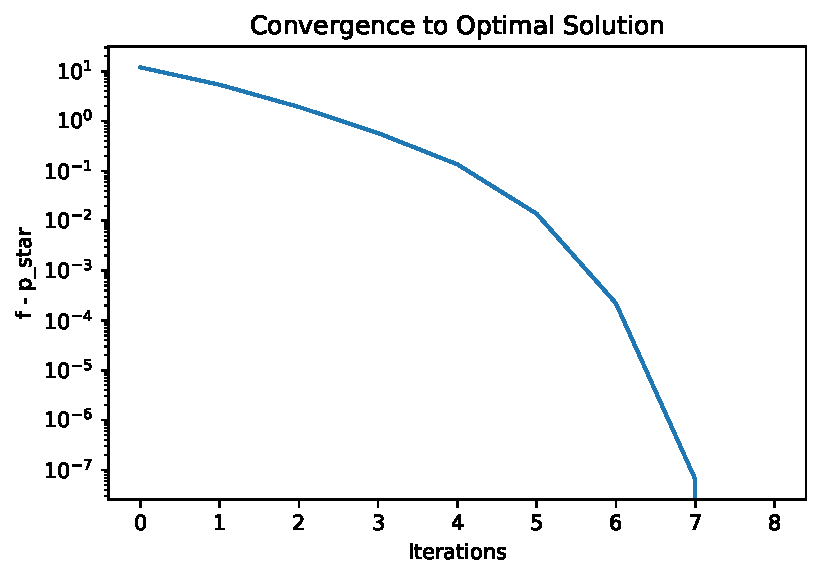
\includegraphics[width= \linewidth]{figures/p3_figure8_1.pdf}

I couldn't get the inseasible Newton method to work on here and
debugging via python is terrible. I am going to implement b and c in
matlab.
\end{document}